

\tikzset{every picture/.style={line width=0.75pt}} %set default line width to 0.75pt        

\begin{tikzpicture}[x=0.75pt,y=0.75pt,yscale=-1,xscale=1]
	\fontsize{12pt}{12pt}\selectfont
	%uncomment if require: \path (0,222); %set diagram left start at 0, and has height of 222
	
	%Image [id:dp8920955941242417] 
	\draw (88.6,111.6) node  {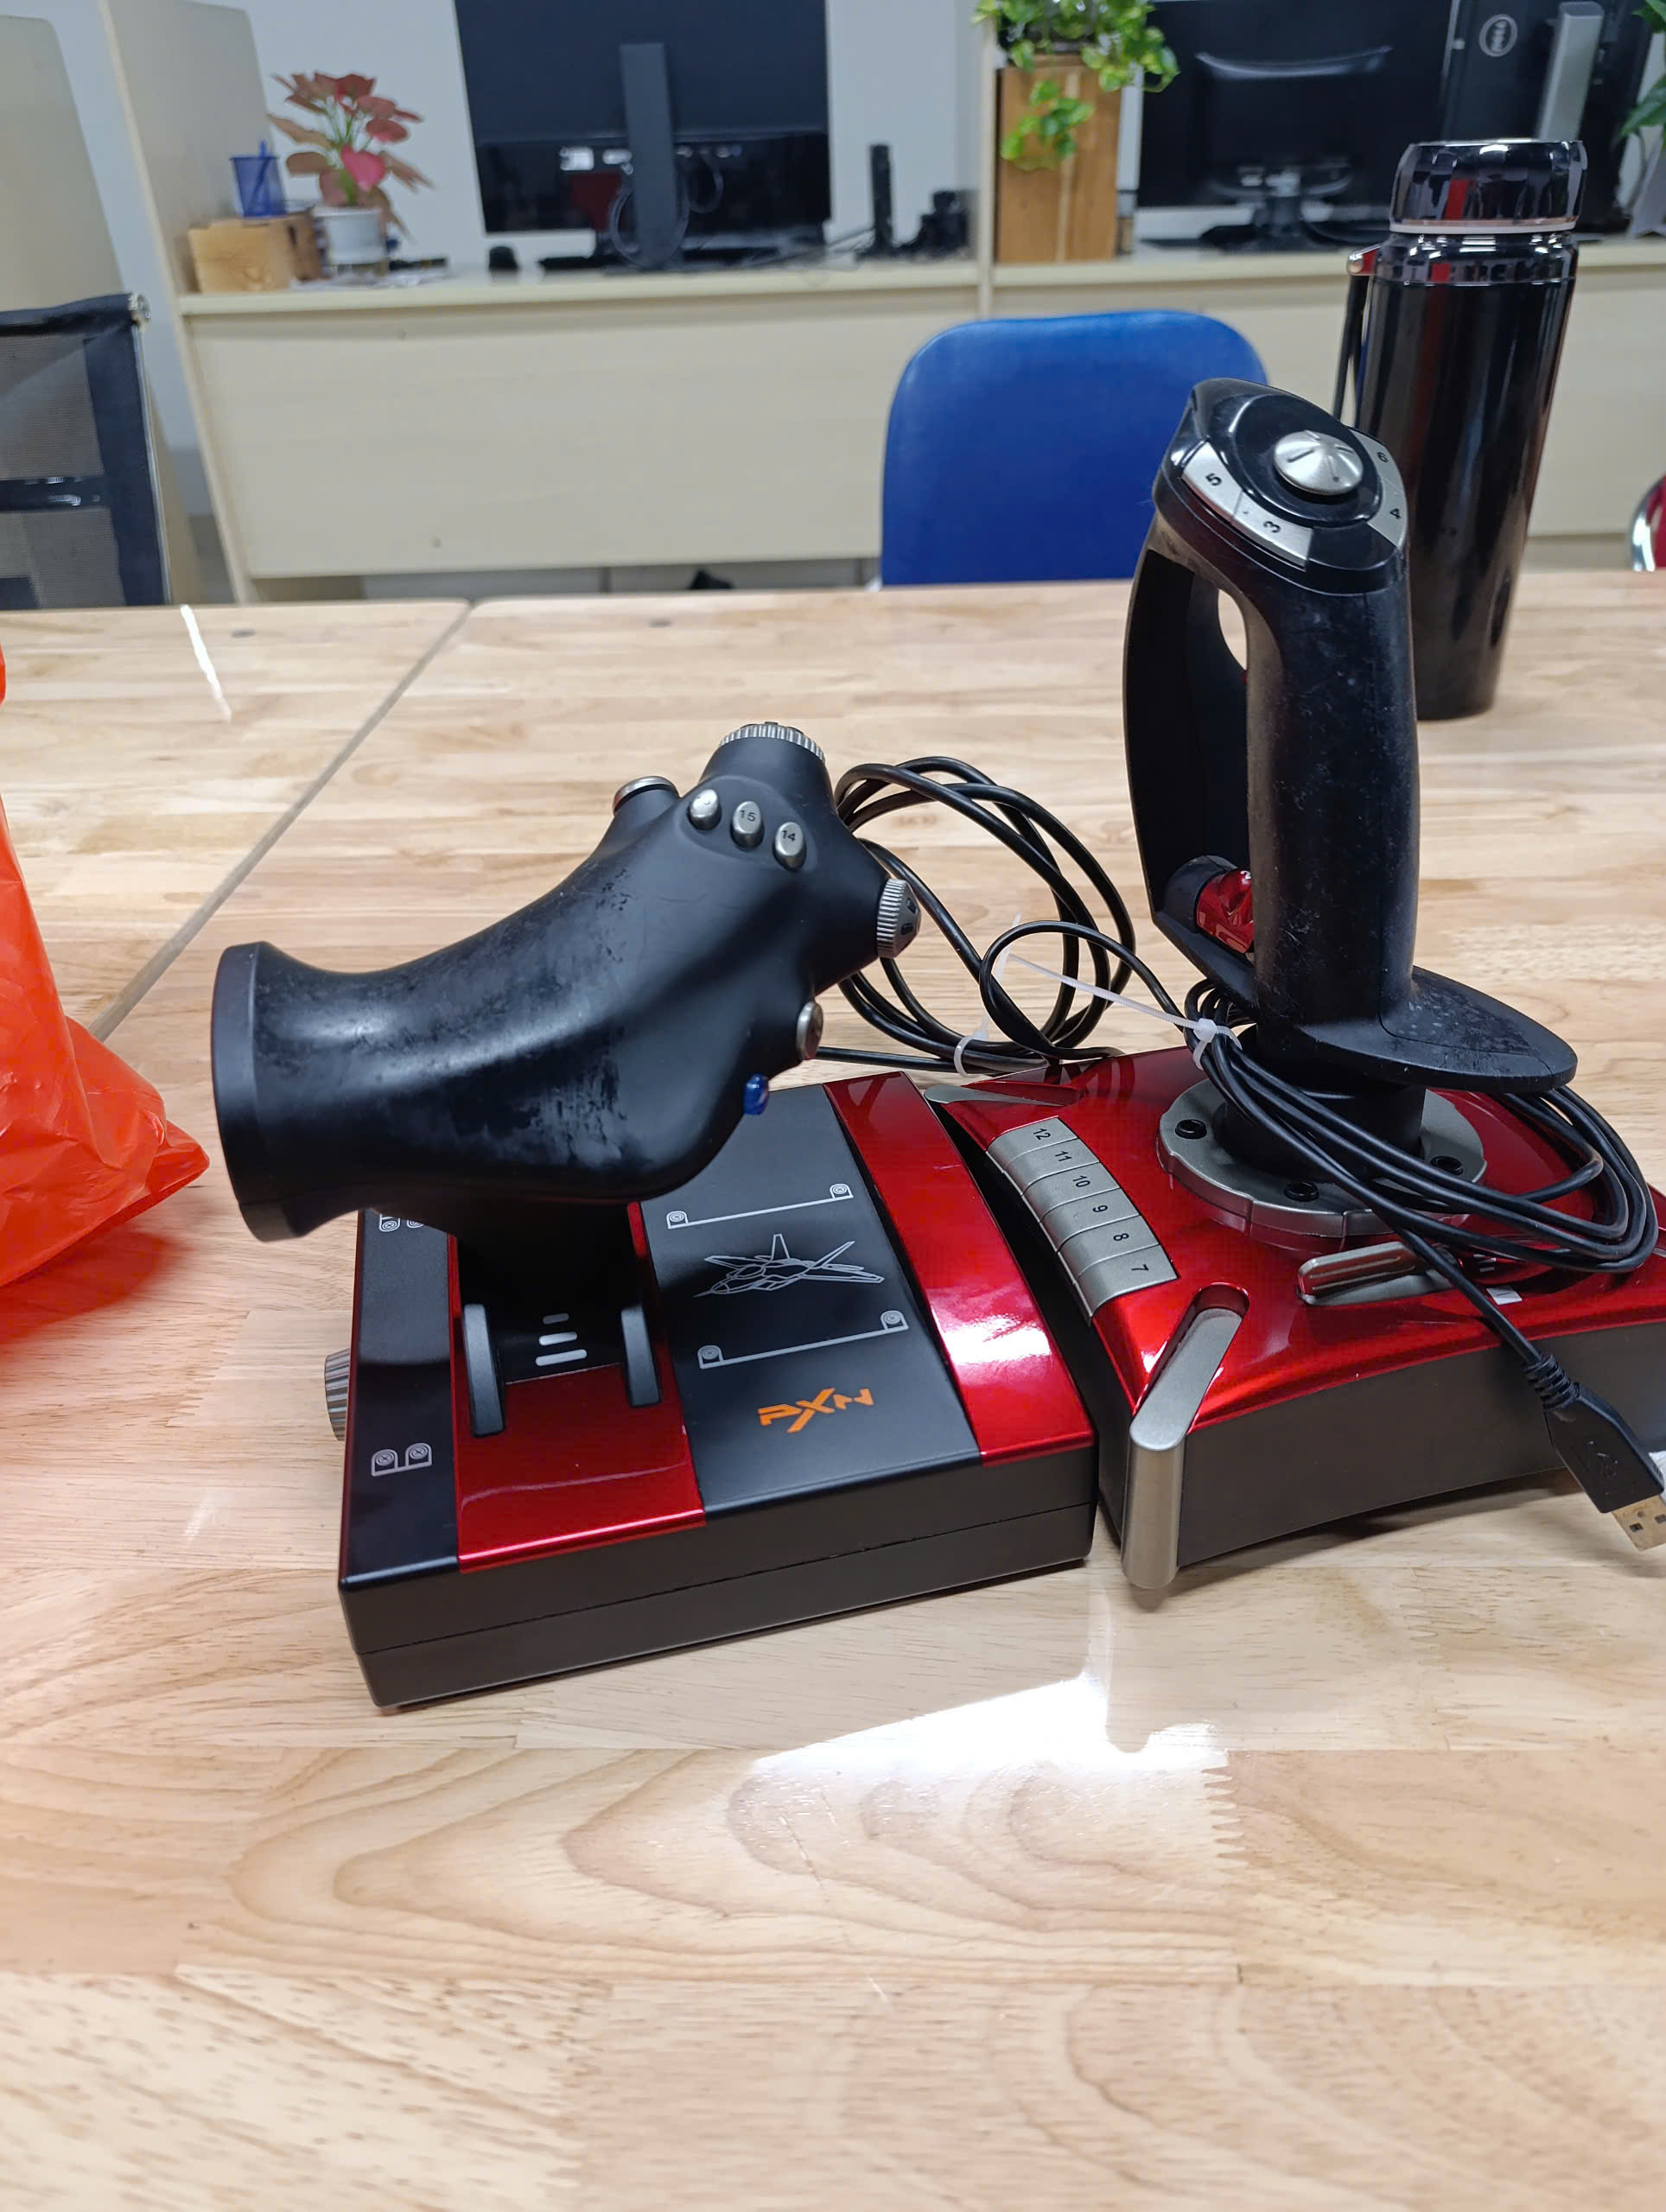
\includegraphics[width=99.91pt,height=99.91pt]{joystick.jpg}};
	%Image [id:dp8812698464016249] 
	\draw (521,112.74) node  {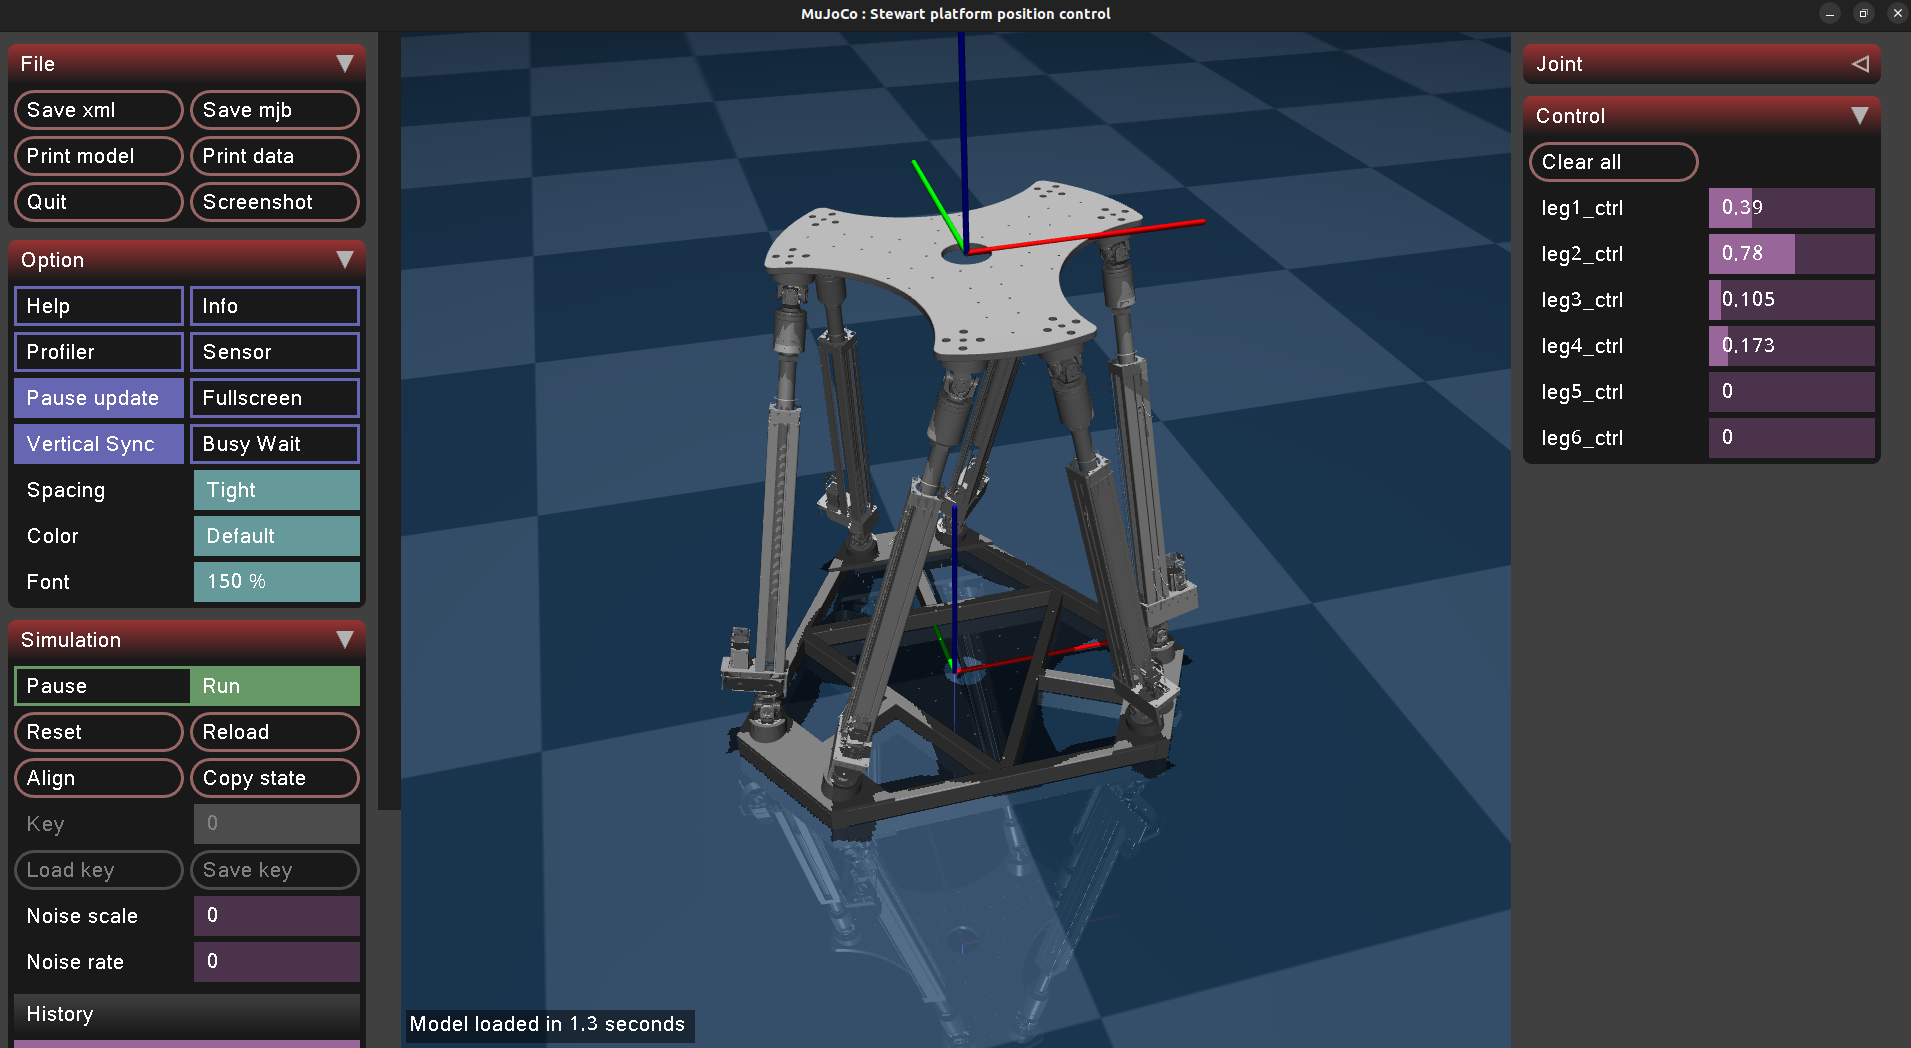
\includegraphics[width=193.5pt,height=106.12pt]{mujoco-stewart.png}};
	%Shape: Rectangle [id:dp8198074648376453] 
	\draw   (392,42) -- (650,42) -- (650,183.49) -- (392,183.49) -- cycle ;
	
	%Right Arrow [id:dp25296009649592344] 
	\draw   (234,146.55) -- (303,146.55) -- (303,140) -- (330,153.1) -- (303,166.21) -- (303,159.66) -- (234,159.66) -- cycle ;
	
	% Text Node
	\draw (180,52) node [anchor=north west][inner sep=0.75pt]   [align=left] {read data from flight joystick};
	% Text Node
	\draw (182,78) node [anchor=north west][inner sep=0.75pt]   [align=left] {evdev};
	% Text Node
	\draw (182,100) node [anchor=north west][inner sep=0.75pt]   [align=left] {pygame};
	
	
\end{tikzpicture}